\documentclass[letterpaper,12pt,fleqn]{article}
\usepackage{matharticle}
\usepackage{tikz}
\pagestyle{plain}
\begin{document}
Cavallaro, Jeffery \\
Math 231a \\
Homework \#0

\bigskip

\begin{enumerate}
\item \(A=\set{1,2,3}\qquad B=\set{1,3,4}\)
  \begin{gather*}
    A\cap B=\set{1,3} \\
    A\cup B=\set{1,2,3,4}
  \end{gather*}

\item How many different ways?
  \begin{enumerate}
  \item Arrange 5 people in a row:
    \[5!=5\cdot4\cdot3\cdot2\cdot1=120\]
  \item Select 4 people from a group of 10:
    \begin{align*}
      \binom{10}{4} &= \frac{10!}{4!(10-4)!} \\
      &= \frac{10!}{4! 6!} \\
      &= \frac{10\cdot9\cdot8\cdot7}{4\cdot3\cdot2\cdot1} \\
      &= 5\cdot3\cdot2\cdot7 \\
      &= 210
    \end{align*}
  \end{enumerate}

\item \(\displaystyle f(x)=\frac{1}{1+\sqrt{x}}\)
  \begin{gather*}
    \text{Domain:}\ x\in[0,\infty) \\
    \text{Range:}\ x\in(0,1]
  \end{gather*}

\item Solve:

  \begin{minipage}{3.25in}
    \begin{gather*}
      -1 < \frac{3-x}{2} < 2 \\
      -2 < 3-x < 4 \\
      -4 < x-3 < 2 \\
      -1 < x < 5 \\
    \end{gather*}
    \[x\in(-1,5)\]
  \end{minipage}
  \begin{minipage}{3.25in}
    \begin{gather*}
      x^2 < 4 \\
      x^2-4 < 0 \\
      (x+2)(x-2) < 0
    \end{gather*}
    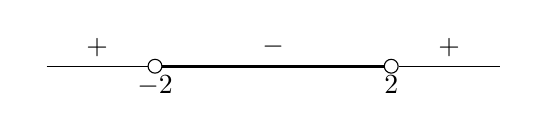
\begin{tikzpicture}
      \node (a) at (-3,0) {};
      \node (b) [draw,circle,inner sep=0pt, minimum size=5pt] at (-1.5,0) {};
      \node (c) [draw,circle,inner sep=0pt, minimum size=5pt] at (1.5,0) {};
      \node (d) at (3,0) {};
      \draw (a) to node [above] {\(+\)} (b);
      \draw [very thick] (b) to node [above] {\(-\)} (c);
      \draw (c) to node [above] {\(+\)} (d);
      \node [below] at (b) {\(-2\)};
      \node [below] at (c) {\(2\)};
    \end{tikzpicture}
    \[x\in(-2,2)\]
  \end{minipage}

\item \(\displaystyle\sum_{n=1}^\infty\frac{1}{n^p}\ \text{converges for}\ p>1\)

\item Determine:
  \[\sum_{i=0}^n\binom{n}{i}a^ib^{n-i}=(a+b)^n\]
  \[\sum_{n=0}^\infty r^n=\frac{1}{1-r}\qquad \abs{r}<1\]
  \[\sum_{n=0}^\infty\frac{A^n}{n!}=e^A\qquad A\in\mathbb{R}\]
  \[\sum_{n=1}^\infty\frac{1}{n(n+1)}=\sum_{n=1}^\infty\left(\frac{1}{n}-\frac{1}{1+n}\right)=1-\frac{1}{2}+\frac{1}{2}-
  \frac{1}{3}+\frac{1}{3}-\cdots=1\]

\item Evaluate:
  \begin{enumerate}
  \item
    \begin{align*}
      \int_1^\infty\frac{2}{x^3}dx &= \lim_{b\to\infty}\int_1^b2x^{-3}dx \\
      &= \lim_{b\to\infty}2\left.\left(\frac{x^{-2}}{-2}\right)\right\rvert_1^b \\
      &= \lim_{b\to\infty}\left(-\left.x^{-2}\right)\right\rvert_1^b \\
      &= \lim_{b\to\infty}\left(-\frac{1}{b^2}+1\right) \\
      &= 0 + 1 \\
      &= 1
    \end{align*}

  \item
    \begin{align*}
      \int_0^1x(1-x)^3dx &= \int_0^2x(1-3x+3x^2-x^3)dx \\
      &= \int_0^1(x-3x^2+3x^3-x^4)dx \\
      &= \left.\left(\frac{x^2}{2}-x^3+\frac{3x^4}{4}-\frac{x^5}{5}\right)\right\rvert_0^1 \\
      &= \frac{1}{2}-1+\frac{3}{4}-\frac{1}{5} \\
      &= -\frac{1}{2}+\frac{3}{4}-\frac{1}{5} \\
      &= -\frac{10}{20}+\frac{15}{20}-\frac{4}{20} \\
      &= \frac{1}{20}
    \end{align*}

  \item
    \[\int_0^\infty xe^{-2x}dx\qquad\text{(by parts)}\]

    \begin{tabular}{ll}
      \(u=x\) & \(dv=e^{-2x}dx\) \\
      \(du=dx\) & \(v=-\frac{1}{2}e^{-2x}\)
    \end{tabular}

    \begin{align*}
      \int_0^\infty xe^{-2x}dx &=
      \left.-\frac{1}{2}xe^{-2x}\right\lvert_0^\infty-\int_0^\infty\left(-\frac{1}{2}e^{-2x}\right)dx \\
      &= 0 +\frac{1}{2}\int_0^\infty e^{-2x}dx \\
      &= \frac{1}{2}\left.\left(-\frac{1}{2}e^{-2x}\right)\right\rvert_0^\infty \\
      &= -\frac{1}{4}\left.e^{-2x}\right\rvert_0^\infty \\
      &= -\frac{1}{4}(0-1) \\
      &= \frac{1}{4}
    \end{align*}

  \item
    \begin{align*}
      \int_0^\infty xe^{-x^2}dx &= -\frac{1}{2}\int_0^\infty \left(-2xe^{-x^2}\right)dx \\
      &= -\frac{1}{2}\left.e^{-x^2}\right\rvert_0^\infty \\
      &= -\frac{1}{2}(0-1) \\
      &= \frac{1}{2}
    \end{align*}
  \end{enumerate}

\end{enumerate}

\end{document}
